\section{Introducción a aplicaciones}
\subsection{Misiones SAR}
\begin{frame}{\secname : \subsecname}
  \begin{figure}
    \centering
    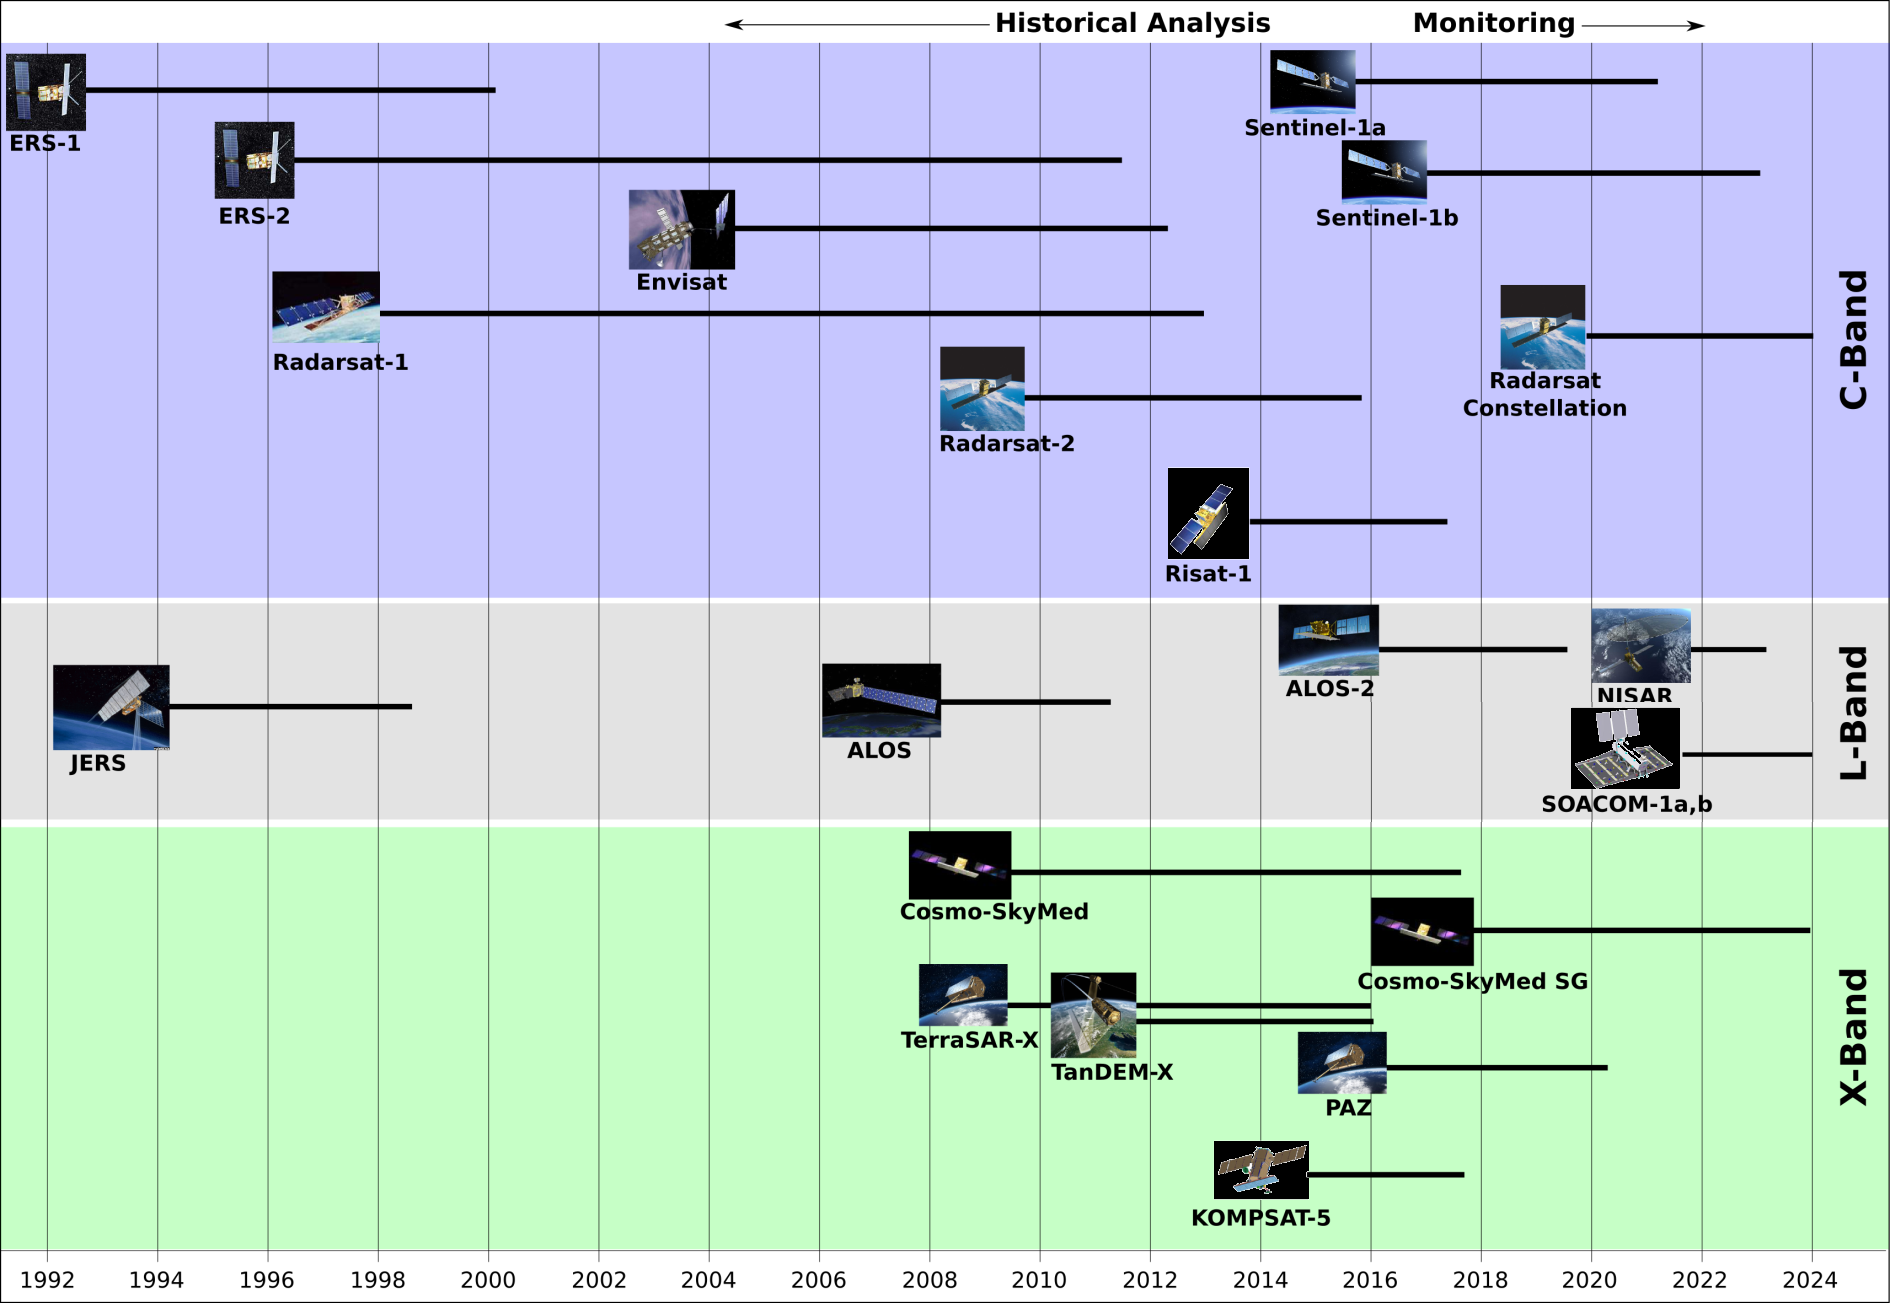
\includegraphics[width=0.7\textwidth]{fig:misiones}
    \caption{Misiones satelitales historicas y actuales.}
    \label{}
  \end{figure}
\end{frame}
%--- Next Frame ---%

\subsection{Plan Espacial Nacional y Serie SAOCOM}
\begin{frame}{\secname : \subsecname}
  \begin{figure}
    \centering
    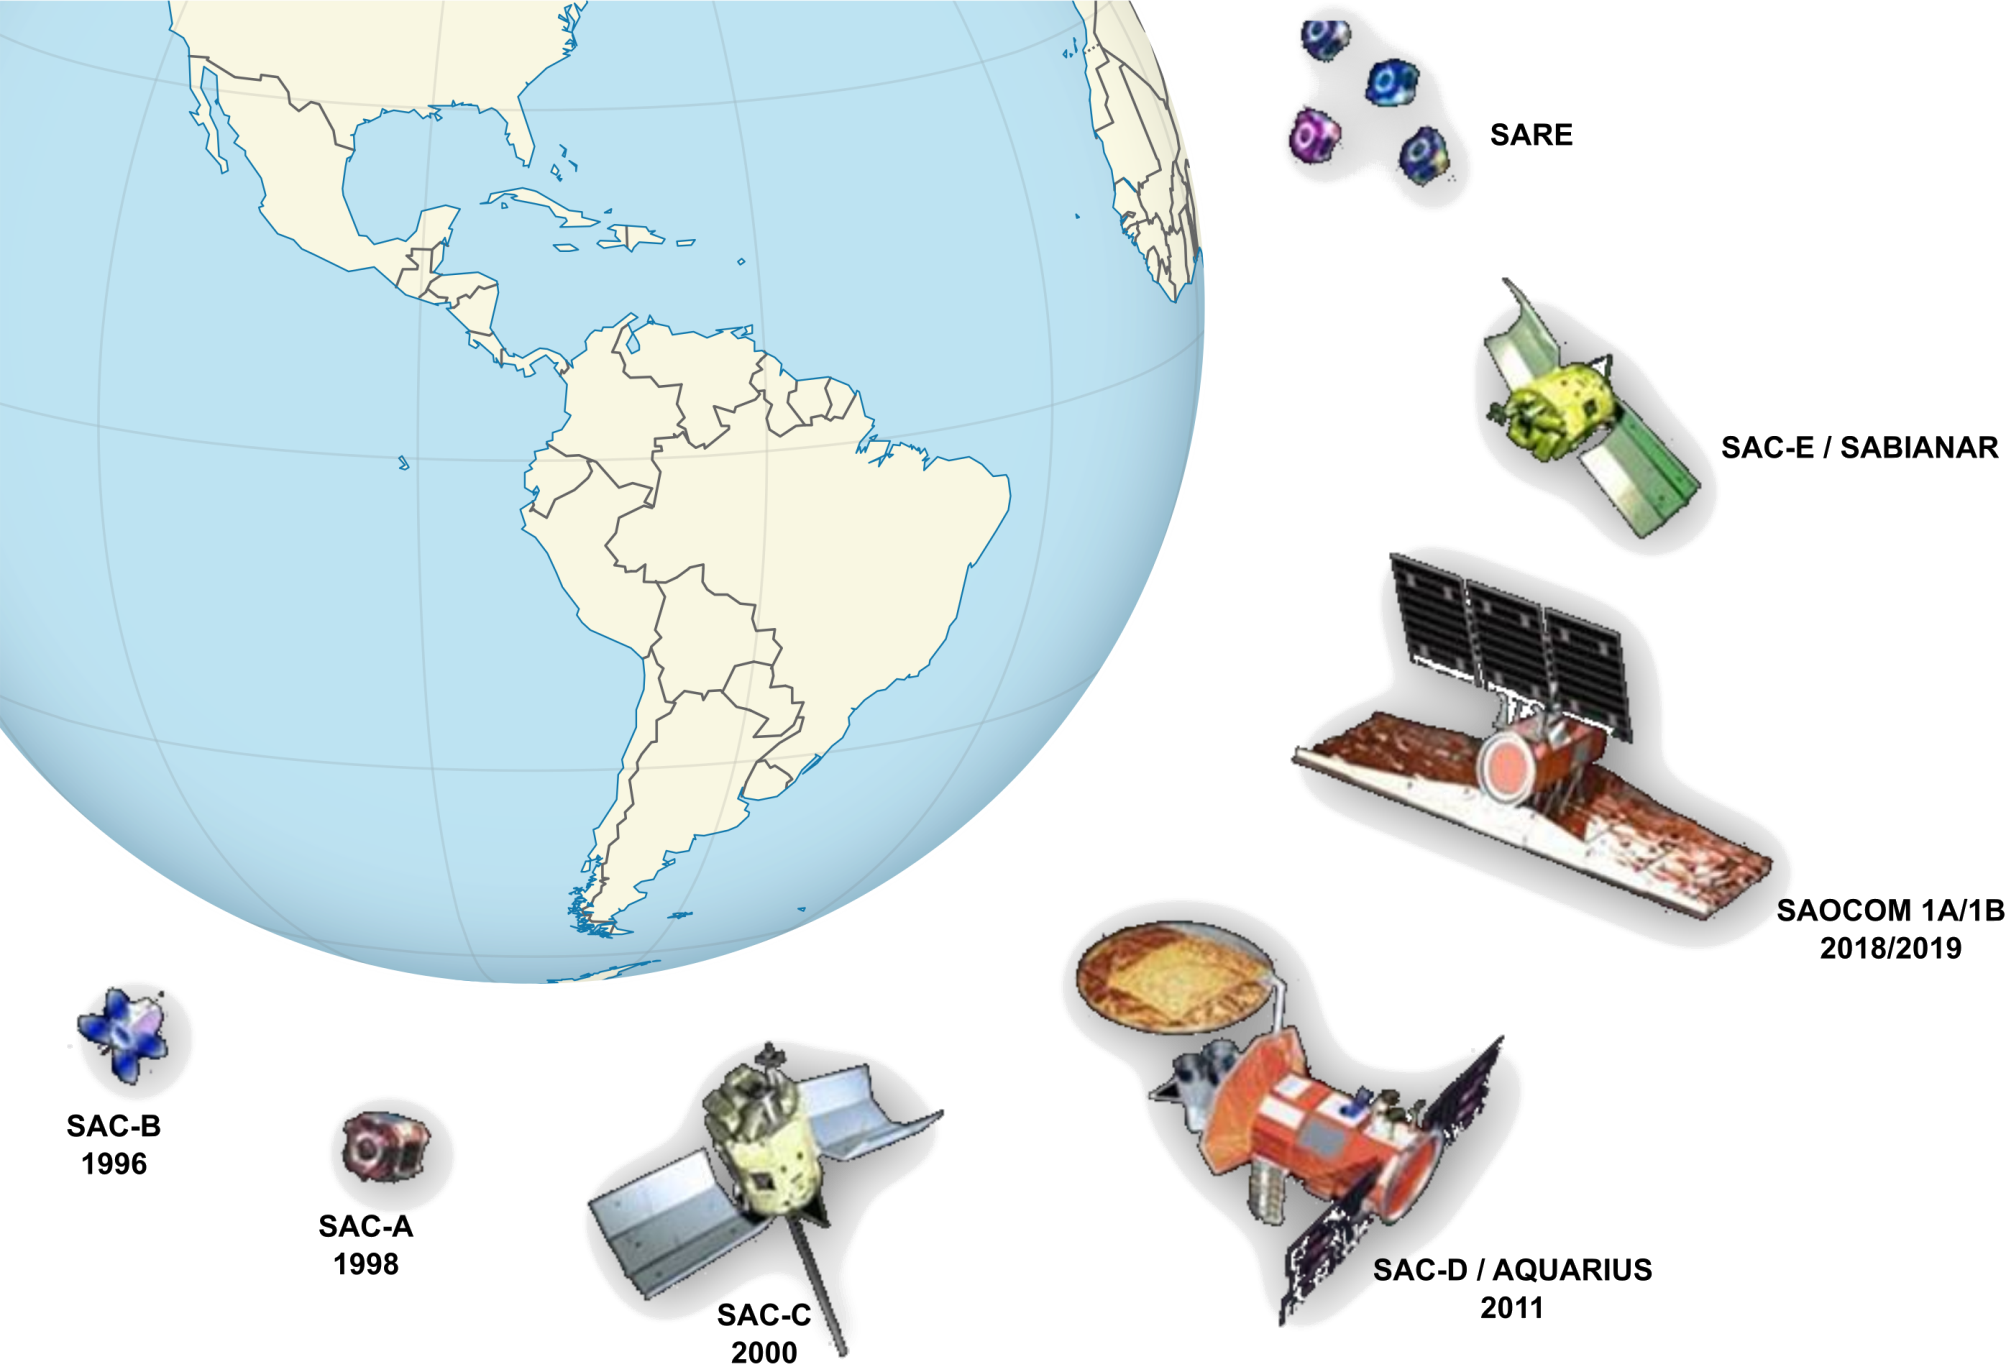
\includegraphics[width=0.65\textwidth]{fig:plan}
    \caption{Satelites del plan espacial nacional.}
    \label{}
  \end{figure}
\end{frame}
%--- Next Frame ---%
\subsection{Serie SAOCOM}

\begin{frame}{\secname : \subsecname}
  \begin{columns}
    \begin{column}{0.6\textwidth}
     \begin{block}{Mision SAOCOM}
\begin{itemize}
  \item Dos satélites idénticos
  \item L-Band SAR (1275 Mhz)
  \item Cobertura Global
  \item Mirada a derecha
  \begin{itemize}
    \item Adquisiciones continuas de 10 minutos en visibilidad de una estación
    \item 15 minutos por órbita en promedio
    \item 20 minutos de adquisiciones no continuas en una órbita
  \end{itemize}
  \item Mirada a izquierda
  \begin{itemize}
    \item Hasta 5 minutos
  \end{itemize}
  \item Antena activa de 10m x 3.5m con 140 MTR
\end{itemize}
     \end{block}
    \end{column}
    \begin{column}{0.4\textwidth}  %%<--- here
      \begin{figure}
        \centering
        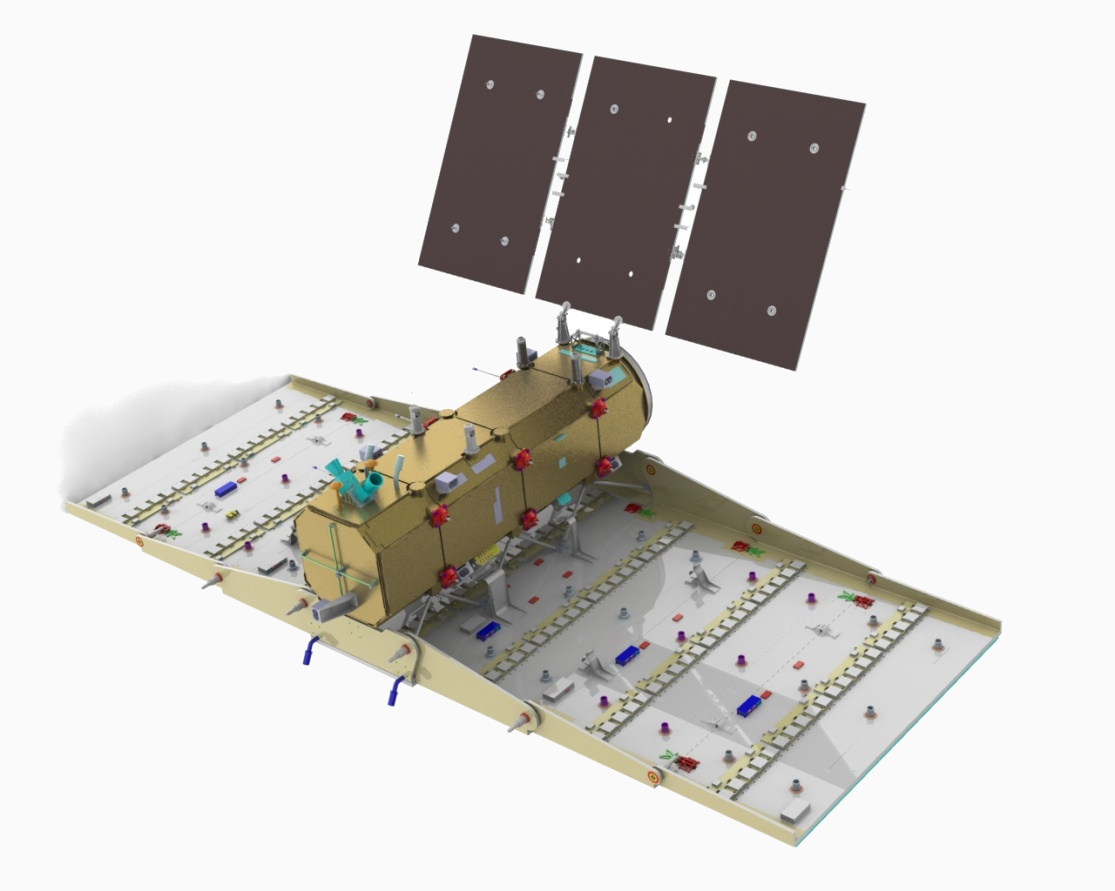
\includegraphics[width=1.1\textwidth]{fig:saocom.jpg}
        \caption*{}
        \label{}
      \end{figure}
    \end{column}
    \end{columns}

\end{frame}
%--- Next Frame ---%


\subsection{Segmento de vuelvo}
\begin{frame}{\secname : \subsecname}
\begin{itemize}
  \item Órbita polar, heliosincrónica (inclinación 97.89) a 620 km de altura
  \item Cada satélite esta desfasado 180 grados
  \item Hora local de pasada por el Ecuador en forma ascendente : 06:12 am
  \item Duración de la orbita 97,2 minutos
  \item Tiempo de revisita: 16 días (1 satélite) / 8 días (constelación)
  \item Orbitas por ciclo: 237
  \item 23 ciclos por año
\end{itemize}
\end{frame}
%--- Next Frame ---%
